%# -*- coding: utf-8-unix -*-
%%==================================================
%% test.tex for SJTU Master Thesis
%%==================================================

%\bibliographystyle{sjtu2}%[此处用于每章都生产参考文献]
\chapter{验证与测试}
\label{chap:test}

本章从功能验证和测试的角度阐述了Fornax的功能与性能。并且通过对于同类型产品的比较,对Fornax的特点进行了说明。

\section{功能性测试}

作为着眼于持续集成、持续发布以及版本管理的系统,Fornax对于代码的质量有严格的保证,其具有完善的测试用例,并使用Jenkins作为持续集成工具,对于每次提交进行持续集成测试,在确保不会引入问题时才会将代码合并。目前Fornax在运行时会依赖数据库组件MongoDB和消息中间件Kafka,而Kafka作为开源的消息中间件实现,本身还会依赖分布式协调一致组件Zookeeper。因此,如果要进行端到端测试,需要先将这三个服务运行,Fornax才能被正确地启动。

\begin{figure}[!htp]
  \centering
  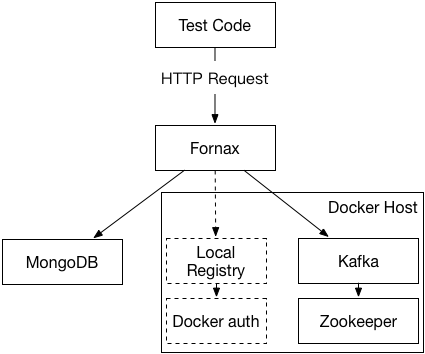
\includegraphics[width=0.55\textwidth]{test/test.png}
  \bicaption[fig:test]{Fornax测试架构图}{Fornax测试架构图}{Fig}{}
\end{figure}

如图\ref{fig:test},Fornax会将Kafka和Zookeeper以Docker容器的方式启动,将数据库启动在本地,除此之外,为了测试版本的推送功能,Fornax需要一个Docker Registry进行验证,而测试的应用场景对于Docker Registry有着不同于平时的需求,其要求Docker Registry的生命周期足够短,在测试结束时不能留下残余垃圾。因此使用公共的或者私有的Docker Registry都不能满足这样的要求,因此在Fornax启动之前,一个私有的Docker Registry会被启动,随之而存在的用以认证的一个服务也会随之启动。这两个服务也是以Docker容器的方式运行的。随后Fornax会被真正地运行,而测试代码是独立于Fornax实例而存在,其本质是模拟Fornax的客户端,对Fornax发起HTTP请求以测试Fornax在行为级别的表现是否满足预期,而针对Fornax的代码,有一些异常路径的测试用例被执行,因此属于端到端的测试,也可以被视为灰盒测试。

目前,Fornax中具有35个端到端的测试用例,覆盖了Fornax的全部的主要流程和部分异常流程。Fornax使用行为驱动的测试风格维护这些测试用例,使得在新增用例时代码不会过于膨胀。在35个测试用例中,有11个用例测试有关服务的逻辑,15个用例测试有关版本中构建与发布的逻辑,还有额外的9个用例专门关于给定配置文件后构建版本时的逻辑。因为在创建版本时版本镜像的构建与发布是默认的行为,因此相比于给定配置文件后进行构建的应用场景要更常见一些,所以书写了更多的测试用例。但从代码复杂度而言,给定配置文件后进行构建要比直接构建与发布镜像要复杂许多,因此在之后Fornax会补充更多完善的关于根据配置文件进行构建的测试用例。

\section{分布式部署}

Fornax作为一个生产环境可用的版本管理与发布的工具,支持分布式的部署方式。Fornax本身是无状态的,因此在分布式的支持上有很多种选择,而Fornax目前采取的方法是使用了第三方的反向代理工具,对Fornax进行请求的代理。Fornax进行分布式部署的目的在于提高系统的可用性以及请求的吞吐量,使得Fornax能够真正成为一个生产环境可用的工具。

\begin{figure}[!htp]
  \centering
  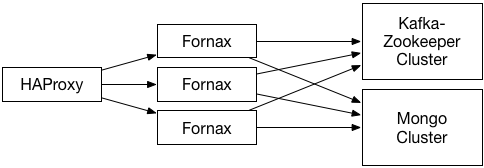
\includegraphics[width=0.55\textwidth]{test/distributed.png}
  \bicaption[fig:distributed]{Fornax分布式部署}{Fornax分布式部署}{Fig}{}
\end{figure}

如图\ref{fig:distributed}所示,Fornax在分布式部署中使用到了HAProxy作为反向代理的工具。在结构上主要分为Fornax集群,Kafka集群和Mongo集群。Fornax集群中每个实例的关系是完全对等的,都是无状态的。而Mongo集群和Kafka集群是使用其默认的分布式部署的支持方式进行部署的,它们为多个Fornax的实例提供服务。每当有请求路由到HAProxy时,HAProxy会根据自身的负载均衡策略将请求分发至一个具体的Fornax实例,该实例收到由其路由过来的请求后,会对其进行处理,并将服务,版本等信息存储到数据库集群中,而有关日志的信息会存储到消息中间件集群中。

在最开始的设计中,Fornax对于日志的处理上是使用本地文件,而不是消息中间件的方式来实现的。这样的实现方式在将Fornax进行分布式部署的尝试时遇到了问题。使用本地文件来存储日志信息使得Fornax本身不是完全无状态的,这要求对于同一个构建,其相关的请求都要路由到同一个Fornax实例上,因为对于构建的日志是存储在实例所在机器的本地的,而这样的分布式部署并不能真正起到提高可用性的目的。因此在后期的实现中Fornax引入了Kafka的依赖,讲日志也持久化在分布式的消息中间件中,所有的Fornax实例都连接该分布式的消息中间件,因此无论客户端请求在哪个Fornax实例上进行构建任务的日志,任意一个Fornax实例都可以订阅Kafka中的主题,来将日志推送给客户端。这样的实现是的Fornax成为了无状态的服务器,所有需要持久化的数据都下沉到了数据库与消息中间件中。而因为Fornax是无状态的,而且所有的实例都使用同一个数据库集群和消息中间件集群,所以连续的请求不需要路由到同一个实例上,这也是Fornax可以采取这样的分布式架构的主要原因。因为Fornax是无服务的,所以在部署时,Fornax实例是以Docker容器的方式运行的。而反向代理工具HAProxy也是以这样的方式进行部署,这使得Fornax的弹性扩容能力与可用性都相比于传统的部署方式有很大的提高,可以面对未来复杂多变的应用环境。

与此同时,Fornax的可配置性好,允许对所有的依赖进行配置,使得依赖由静态变成了动态的过程。同时Docker容器化的部署使得Fornax不感知真实的环境,因此无论是在公有云、私有云亦或是混合云,Fornax都可以进行部署。

% \section{性能测试}

\section{代码统计}

Fornax代码情况使用cloc\supercite{cloc}统计,去除了Fornax中对于其他模块的代码依赖。情况如表\ref{tab:code}所示,Fornax的主要功能由go语言实现,其中包括八个核心的模块,以及所有的测试用例,因此go语言的代码占代码总量的大部分。除此之外,Fornax在启动时有很多的运行时依赖,这些依赖的运行以及Fornax的启动都是通过Bourne Shell脚本来完成的,其中包括启动本地的短生命周期的Docker Registry,启动Fornax,执行端到端的测试等内容。

\begin{table}[!hpb]
  \centering
  \bicaption[tab:code]{指向一个表格的表目录索引}{Fornax代码统计}{Table}{}
  \begin{tabular}{lllll} \toprule
    语言 & 文件数 & 注释 & 代码 \\ \midrule
    Go & 62 & 1129 & 6671 \\
    Bourne Shell & 15 & 96 & 375 \\
    YAML & 11 & 4 & 249 \\
    HTML & 1 & 0 & 31 \\
    make & 1 & 8 & 12 \\ \midrule
    总计 & 90 & 1237 & 7338 \\ \bottomrule
  \end{tabular}
\end{table}

\section{相较于其他工具的优势}

Fornax关注持续集成与持续部署,版本的管理与发布,是两者的结合。在业界,有不少与Fornax具有类似功能的工具,比如Jenkins、Drone、Travis CI等。而这些工具跟Fonnax之间存在着一些功能的差异,以及思想的不同。本节将从这些工具的差别的角度出发介绍Fornax的优势。

Jenkins,Drone,Travis CI都是关注持续集成的工具。它们在实现上各有不同。Jenkins是三个工具当中最早,也是最流行的持续集成工具。其实现并没有借助容器虚拟化的技术,而只是通过操作系统的进程,目录等等进行了简单的隔离。不过Jenkins支持主从结构的分布式部署,经历过真实使用的考验。Jenkins采用Java实现,代码简洁易懂,插件众多,扩展性好。同时,Jenkins提供了网页和API两种方式进行构建,API使用XML格式作为传输格式。因此在配置的可读性上,比以YAML格式的配置文件难以阅读。但这并不影响Jenkins是目前市场份额最大的开源持续集成工具。在Fornax的实现过程中,也是使用Jenkins来对Fornax进行持续集成,保证Fornax的代码质量的。

Drone是一个新兴的持续集成工具,与Fornax一样,是使用go语言实现的,其在持续集成过程的工作流与Fornax类似,都是采取了YAML格式的配置文件来控制整个持续集成流程的方法。Drone本身的目的是取代Jenkins成为持续集成工具的下一代主流,因此就功能而言与Jenkins相差无几。而从实现角度而言,Drone与Fornax相同,使用了Docker来进行构建时的隔离,其同样支持插件,并且有命令行工具支持,可以通过命令行直接与Drone进行交互,完成构建,对于开发者而言更加友好。相比于Jenkins,Drone使用了更多的新技术与新工具,使得代码实现更加简洁的同时,拥有更好地隔离性。Drone也支持分布式的部署,它允许接入多个Docker Host来进行分布式的构建。

Travis CI是另外一款开源的持续集成工具,主要使用Ruby语言实现。Travis CI的功能与前两者并无区别,只是另一种的实现思路。Travis CI对于隔离的方式有更多的选择,并且其在日志传输等方面更加成熟。在其开源的版本中,有使用容器来进行构建隔离的实现。

\begin{table}[!hpb]
  \centering
  \bicaption[tab:advantage]{指向一个表格的表目录索引}{Fornax与其他工具对比}{Table}{}
  \begin{tabular}{l||lllll} \toprule
     & 实现语言 & 持续集成 & 分布式 & 容器隔离 & 版本管理 \\ \midrule
    Jenkins & Java & 支持 & 支持 & 不支持 & 不支持 \\
    Drone & Golang & 支持 & 支持 & 支持 & 不支持 \\
    Travis CI & Ruby & 支持 & 支持 & 支持 & 不支持 \\
    Fornax & Golang & 支持 & 支持 & 支持 & 支持 \\ \bottomrule
  \end{tabular}
\end{table}

Fornax与其他工具的对比如表\ref{tab:advantage}所示,Fornax也如其他工具一样,具有持续集成的功能,并且使用了容器虚拟化技术对构建进行隔离,保证构建之间互相不感知。Fornax可以通过HAProxy来进行分布式的部署,以满足更高的吞吐量要求。而Fornax不仅是一个专注于持续集成的工具,同样是一个版本管理与发布的平台。对于其他的持续集成工具,每次构建只会留下日志。而对于Fornax而言,不仅日志会保留,每次构建在成功时还会构建并且发布一个版本镜像,这也是Fornax与其他的持续集成工具最大不同所在。而且Fornax在解决发布的问题上与其他的工具也存在不同。Fornax目前是一个专用性的工具,只关注将应用部署到Kubernetes集群上。这意味着Fornax可以根据这样的应用场景做适配与优化。

因此,Fornax在定位上与现有的持续集成工具存在一定的差异,持续集成不是Fornax唯一的功能,相比于其他的持续集成工具,Fornax更加关注对于版本的管理,以及将应用部署到容器集群上的过程。这也是Fornax的优势所在。